% XCircuit output "noisea.tex" for LaTeX input from noisea.eps
\def\putbox#1#2#3#4{\makebox[0in][l]{\makebox[#1][l]{}\raisebox{\baselineskip}[0in][0in]{\raisebox{#2}[0in][0in]{\scalebox{#3}{#4}}}}}
\def\rightbox#1{\makebox[0in][r]{#1}}
\def\centbox#1{\makebox[0in]{#1}}
\def\topbox#1{\raisebox{-0.60\baselineskip}[0in][0in]{#1}}
\def\midbox#1{\raisebox{-0.20\baselineskip}[0in][0in]{#1}}
   \scalebox{1}{
   \normalsize
   \parbox{7.58333in}{
   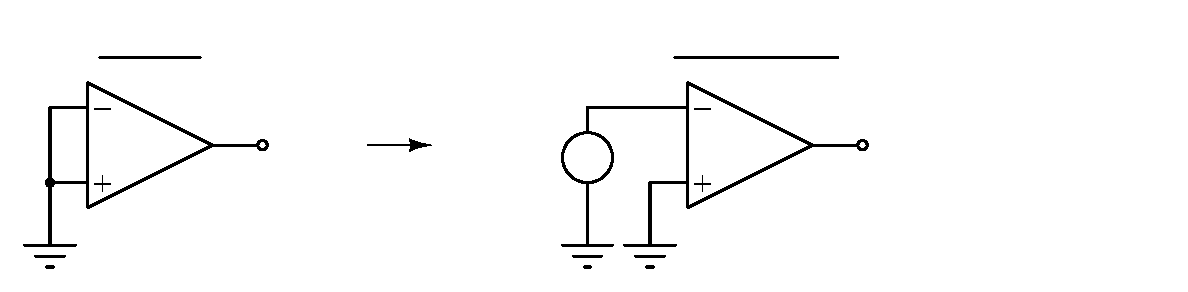
\includegraphics[scale=1]{noisea.eps}\\
   % translate x=496 y=348 scale 0.38
   \putbox{1.81in}{0.79in}{1.20}{$\overline{V_{n}}^2$}%
   \putbox{3.06in}{0.70in}{1.20}{$\overline{V_{n,i}}^2$}%
   \putbox{5.72in}{0.79in}{1.20}{$\overline{V_{n}}^2$}%
   \putbox{0.64in}{1.54in}{1.20}{Noisy}%
   \putbox{4.47in}{1.54in}{1.20}{Noiseless}%
   } % close 'parbox'
   } % close 'scalebox'
   \vspace{-\baselineskip} % this is not necessary, but looks better
